\documentclass[12pt,letterpaper]{report}
\usepackage{pgf, tikz}
\usetikzlibrary{arrows, mindmap,graphs,automata,shapes.geometric}
\usetikzlibrary{positioning}
\newcommand{\deriv}[2]{\ensuremath{\frac{\partial #1}{\partial #2}}}

\begin{document}

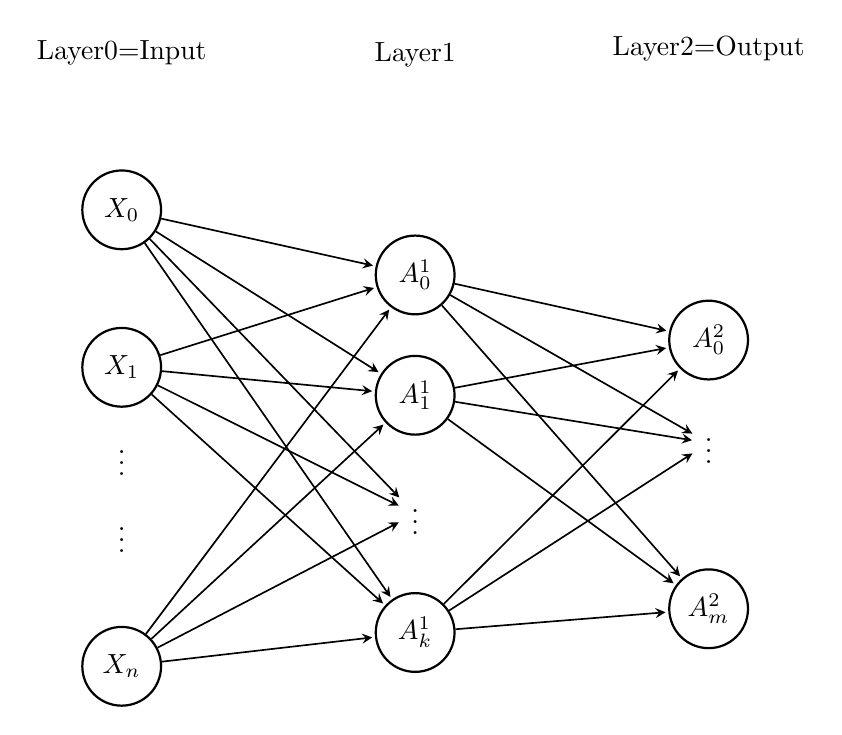
\begin{tikzpicture}[
    > = stealth, % arrow head style
    shorten > = 1pt, % don't touch arrow head to node
    auto,
    node distance = 2cm, % distance between nodes
    semithick % line style
]

\tikzstyle{every state}=[
    draw = black,
    thick,
    fill = white,
    minimum size = 10mm
]

\node[state] (X0) {$X_0$};
\node (input)[above of=X0] {Layer0=Input};

\node[state] (X1) [below of=X0] {$X_1$};
\node (dots) [below=0.2cm of X1] {$\vdots$};
\node (dots2) [below=0.2cm of dots] {$\vdots$};

\node[state] (Xn) [below=0.8cm of dots2] {$X_n$};
\node[state] (A10) [below right=0.1cm and 3cm of X0] {$A^1_0$};
\node[state] (A11) [below=0.5cm  of A10] {$A^1_1$};

\node (layer1)[above=2cm of A10] {Layer1};


\node (dots3) [below=0.6cm of A11] {$\vdots$};
\node[state] (A1k) [below=0.6cm of dots3] {$A^1_k$};
\node[state] (A20) [below right=0.1cm and 3cm of A10] {$A^2_0$};

\node (layer2)[above=2.9cm of A20] {Layer2=Output};

\node (dots5) [below=0.4cm of A20] {$\vdots$};

\node[state] (A2m) [below=1.2cm of dots5] {$A^2_m$};
\path[->] (X0) edge (A10);
\path[->] (X0) edge (A11);
\path[->] (X0) edge (dots3);
\path[->] (X0) edge (A1k);

\path[->] (X1) edge (A10);
\path[->] (X1) edge (A11);
\path[->] (X1) edge (dots3);
\path[->] (X1) edge (A1k);
\path[->] (Xn) edge (A10);
\path[->] (Xn) edge (A11);
\path[->] (Xn) edge (dots3);
\path[->] (Xn) edge (A1k);

\path[->] (A10) edge (A20);
\path[->] (A10) edge (A2m);
\path[->] (A10) edge (dots5);
\path[->] (A11) edge (A20);
\path[->] (A11) edge (A2m);
\path[->] (A11) edge (dots5);

\path[->] (A1k) edge (A20);
\path[->] (A1k) edge (A2m);
\path[->] (A1k) edge (dots5);
% \path[->] (X0) edge node[at start, anchor=west,yshift=10pt] {$w^1_{00}$} (A10) ;
% \path[->] (X0) edge node[at start, anchor=north west,xshift=5pt,yshift=6pt] {$w^1_{0k}$} (A1k) ;

% \path[->] (X1) edge node[at start,anchor=west,yshift=10pt] {$w^1_{10}$} (A10) ;

% \path[->] (X1) edge node[at start,anchor=west] {$w^1_{1k}$} (A1k) ;
% \path[->] (Xn) edge node[at start, anchor=north,xshift=4pt,yshift=30pt] {$w^1_{n0}$} (A10) ;
% \path[->] (Xn) edge node[at start, anchor=north,xshift=10pt] {$w^1_{nk}$} (A1k) ;

\end{tikzpicture}
\end{document}
